\subsubsection{04.03.2016}
\textit{\textbf{Time frame:}} 17:00-21:00 

Today it was created the cascade of furniture slats for lifting mechanism (figure \ref{Elevator4.6}< \ref{Elevator4.7}). It consisted of three pairs of 35 cm slats placed at the angle of $90^circ$. The construction was created using thin slats (150 g), so the whole assembly weighed only 1,5 kg instead of 3 kg in previous lifting mechanism.

\begin{figure}[H]
	\begin{minipage}[h]{1\linewidth}
		\center{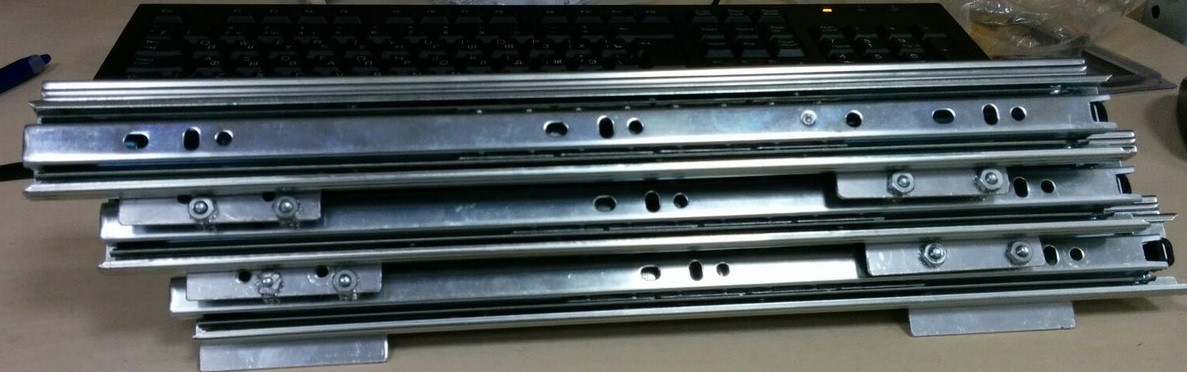
\includegraphics[scale=0.3]{3Engineering/5Team_meetings/days_of_meetings/2016.03.04/images/01}}
		\caption{Cascade of slats (side)}
		\label{Elevator4.6}
	\end{minipage}
	\vfill
	\begin{minipage}[h]{1\linewidth}
		\center{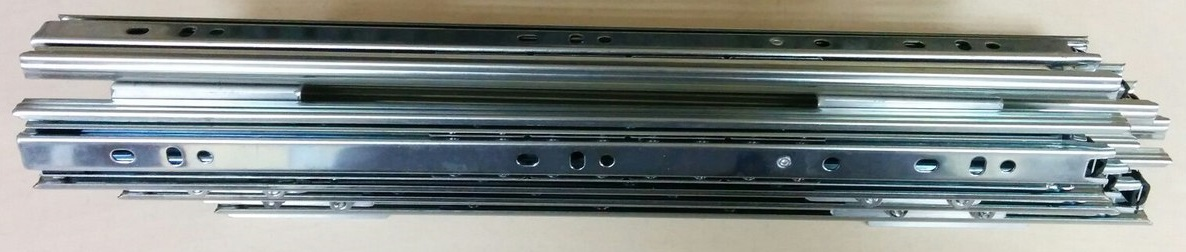
\includegraphics[scale=0.3]{3Engineering/5Team_meetings/days_of_meetings/2016.03.04/images/02}}
		\caption{Cascade of slats (top)}
		\label{Elevator4.7}
	\end{minipage}
\end{figure}
